\subsection{Prose Backend}\label{sec:prose} %0.5p
\begin{figure}[t]
\centering
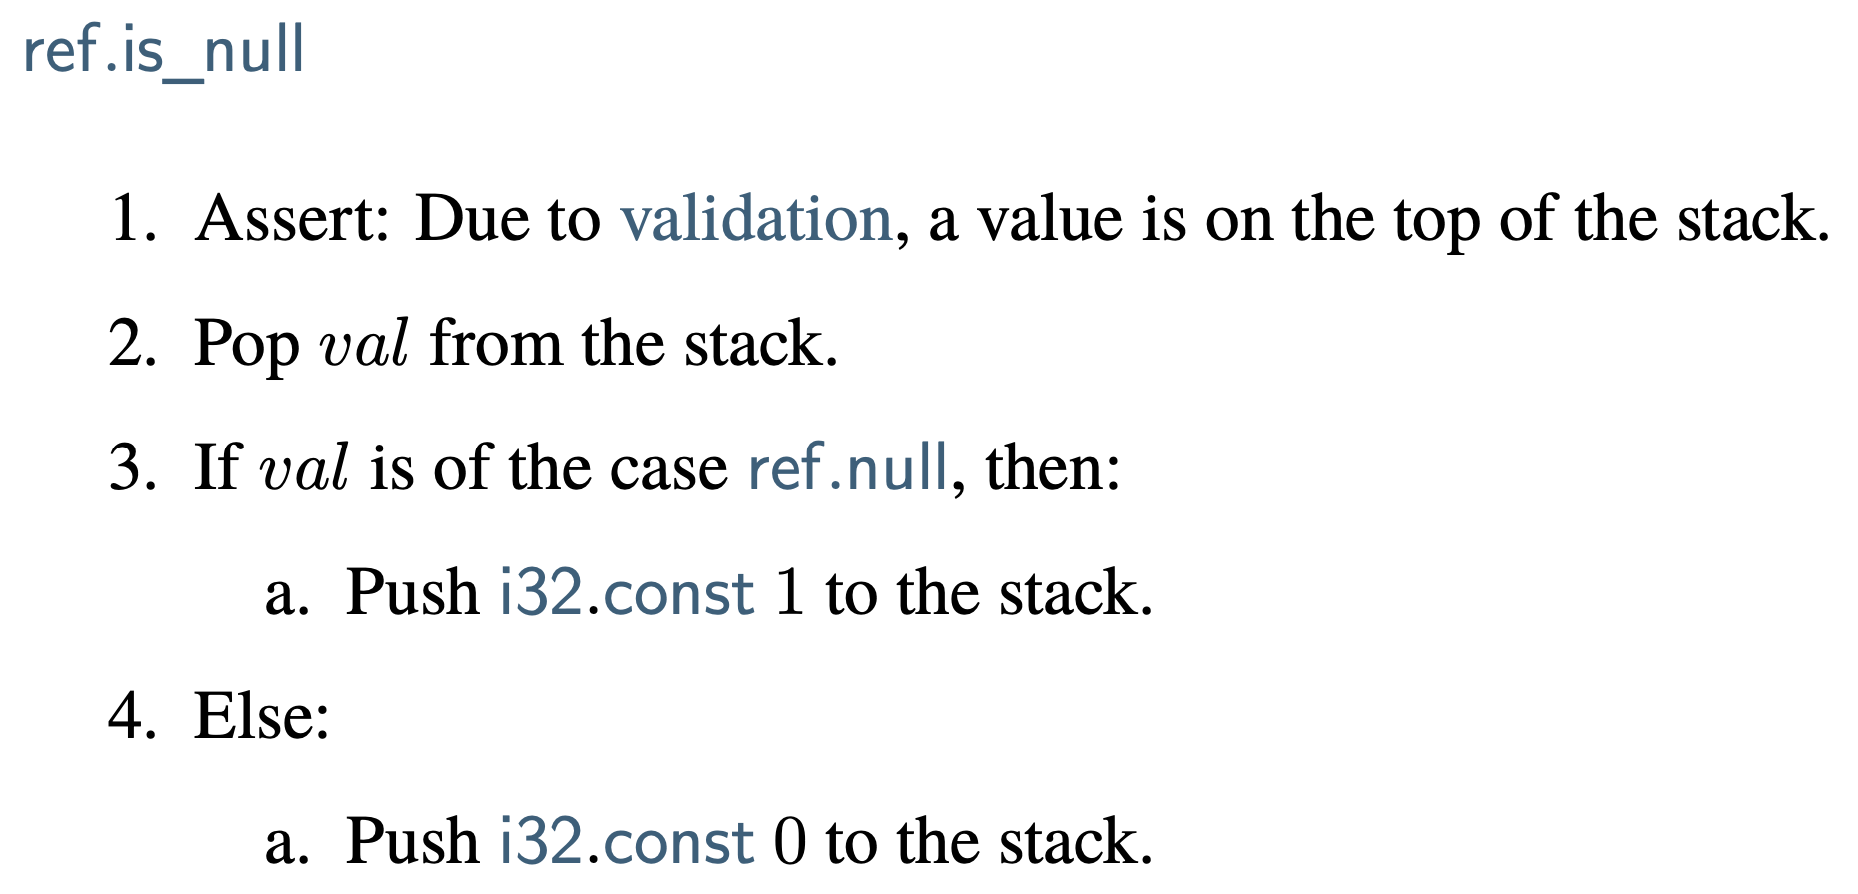
\includegraphics[width=.5\textwidth]{../img/genprose}
\vspace*{-1em}
\caption{Semantics of \inblue{\ensuremath{\mathsf{ref.is\_null}}} in a generated prose specification}
\label{fig:genprose}
\end{figure}

As \al is designed to resemble prose notation, 
generating the English prose specification from \al algorithms is a straightforward task.
Fig.~\ref{fig:genprose} shows the prose pseudocode of \inblue{\ensuremath{\mathsf{ref.is\_null}}} instruction,
generated from the specification in Fig.~\ref{fig:dsl},
which is very close to the original handwritten prose in Fig~\ref{fig:spec1}.
AL algorithms are rendered into prose specification document through three steps.
First, the semantics described in \al is printed into English prose in reStructuredText markup.
For example, the third step of \inblue{\ensuremath{\mathsf{ref.is\_null}}} is printed as follows:
\begin{verbatim}
3. If :math:`val` is of the case \
   :math:`\xref{exec/runtime}{syntax-ref}{\mathsf{ref{.}null}}`, then:
\end{verbatim}
Next, as in the LaTeX backend, prose in reStructuredText are spliced into a skeleton specification document.
Finally, the spliced document is processed by the Sphinx documentation tool~\cite{sphinx},
producing human-frieldnly formats like PDF and HTML.

Note that prose in reStructuredText is not simple plaintext,
but has inline math blocks as denoted by the \texttt{:math:} markup.
Expressions in math blocks are typesetted with LaTeX, thereby
making a clear distinction between specification elements and ordinary English phrases.
Furthermore, the prose backend embeds cross-references into the math blocks 
with \texttt{\textbackslash xref\{doc\}\{section\}\{text\}}.
This serves as a reference to a \texttt{section}
in some reStructuredText file \texttt{doc}, to be rendered as \texttt{text}.
As in the original specification document, 
\inblue{\ensuremath{\mathsf{ref{.}null}}} in the third step references its syntax production rule in a separate file.
This systematic insertion of references rules out
possibilities of missing, broken, or misplaced links when inserted manually.
